\documentclass{article}
\usepackage[utf8]{inputenc}
\usepackage{graphicx}
\usepackage{color}

\newenvironment{text-blue}{\color{blue}}{}
\newenvironment{text-red}{\color{red}}{}

\begin{document}

\title{Classificação de ruído em biosinais \\ Trabalho prático nº2, Computação Adaptativa}
\author{Adriano Vinhas (2009106560, avinhas@student.dei.uc.pt)\\
		José Ribeiro (2008112181, jbaia@student.dei.uc.pt}
\maketitle
\clearpage

% Introdução
\section{Introdução}

\indent \indent Este trabalho, no âmbito da disciplina de Computação Adaptativa, tem como objectivo construir uma rede neuronal multimacamada capaz de reconhecer se um sinal biológico deve ser descartado (devido à presença de ruído) ou deve ser analisado. Este reconhecimento é feito com base num conjunto de características do sinal que vão servir de entrada para a rede neuronal.

Este objectivo foi atingido fazendo um estudo paramétrico tendo em conta os seguintes parâmetros de estudo:
\begin{itemize}
\item Método de treino
\item Coeficiente de aprendizagem
\item Número de neurónios na camada escondida
\item Dimensionalidade do problema
\item Número de épocas do treino
\item Aplicação de normalização sobre os dados
%\item Goal (Erro de treino) ???
\end{itemize}

A parte que foi mais focada na realização deste trabalho foi o estudo paramétrico feito com base nos parâmetros acima indicados. Com base nos resultados obtidos, procurámos uma solução que nos permitisse chegar à combinação dos parâmetros que optimizasse os valores de sensibilidade e especificidade das saídas da rede.

\clearpage
\section{Concepção da rede neuronal}
\indent \indent Nesta secção estão descritas a arquitectura da rede usada para o trabalho e a forma como foi feito o treino da rede.

A arquitectura da rede neuronal usada para o trabalho prático caracteriza-se por 26 entradas e 1 saída, sendo que cada uma das entradas representa uma característica do \textit{dataset} que nos foi fornecido e a saída representa a decisão (se o sinal deve ser descartado ou analisado). No entanto, para os testes efectuados, o número de entradas da rede está sujeito a alterações, sendo este número dependente do uso (ou não) de mecanismos de redução de dimensionalidade.

A função de activação usada para a camada interna foi a tangente hiperbólica, para garantir que a rede neuronal pudesse ser um aproximador universal, e para a camada de saída foi usada uma função linear.

A figura~\ref{nn_architecture} representa a arquitectura da rede usada.

\begin{figure}[!h]
  \centering
  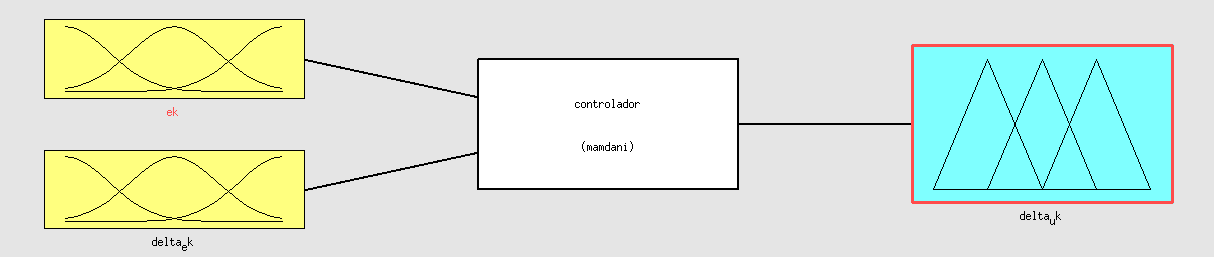
\includegraphics[width=3in]{figures/nn_architecture}
  \caption{Arquitectura da rede usada (com 26 características e 15 neurónios na camada escondida)}
  \label{nn_architecture}
\end{figure}

O \textit{dataset} usado para este trabalho é composto por um total de 12331 exemplos. Deste conjunto, 70\% dos exemplos (8632) foram usados para treinar a rede, e os restantes 30\% (3699) para validação desta e análise de resultados.

O método de selecção de exemplos para cada um dos conjuntos é aleatório. Para que tal aconteça, todos os exemplos são "baralhados" e ficam dispostos numa ordem completamente à ordem original. De seguida é feita a separação segundo a regra 70/30, tal como enunciado acima.

\clearpage
% Gráficos com os resultados. Análise e interpretação.
\section{Estudo paramétrico}
\indent \indent Nesta secção é explicada a metodologia de testes seguida para levar a cabo são apresentados os resultados do estudo paramétrico efectuado para obtenção do resultado óptimo encontrado.

Neste estudo, a ordem dos parâmetros testados torna-se fulcral para melhor explorar o espaço de combinações sem o fazer de forma exaustiva. No fim de cada variação paramétrica, o valor que optimizava as métricas usadas para medir a performance da rede neuronal era fixado na variação paramétrica seguinte. Por exemplo, após a determinação do número óptimo de neurónios para a camada escondida, esse valor era fixado para os restantes testes.

No caso do estudo do coeficiente de aprendizagem, tal não se aplica uma vez que este foi o primeiro parâmetro a ser variado.

Dado o impacto dos variados parâmetros consoante o método de treino, escolhemos efectuar todas as variações paramétricas fixando o método. Como tal, todos os testes relativos a \texttt{trainlm} foram executados separadamente dos testes relativos a \texttt{traingd}.

Para garantir significado estatístico nos resultados, as métricas de avaliação da rede neuronal (performance, sensibilidade e especificidade) apresentadas são a \textbf{média} de \textbf{30} execuções distintas.

A tabela~\ref{study_parameters} sumaria os parâmetros e com valores \textit{default}.

\begin{table}[!h]
\centering
	\caption{Parâmetros predefinidos usados para o estudo paramétrico}
	\label{study_parameters}
	\begin{tabular}{|c|c|}
		\hline 
		\textbf{Parâmetro} & \textbf{Valor utilizado} \\ 
		\hline 
		Coeficiente de Aprendizagem & Não aplicável \\ 
		\hline 
		Neurónios da Camada Escondida & 5 \\ 
		\hline 
		Número de características & 4 \\ 
		\hline 
		Número de épocas de treino & 100 \\ 
		\hline 
		Normalização de input & Com \\ 
		\hline 
	\end{tabular} 
	%\vspace{-1cm}
\end{table}

\subsection{Coeficiente de aprendizagem}
\indent \indent Uma vez que o treino de Levenberg-Marquardt usa um Coeficiente de Aprendizagem adaptativo, este parâmetro apenas se aplica ao método de treino do Gradiente Descendente.

Assim, para o \texttt{traingd}, foram usados os seguintes valores de Coeficientes de Aprendizagem: 0.001, 0.0001 e 0.00001, sendo os restantes valores atribuídos como previamente indicado.

Como tal, o melhor resultado registou-se para o valor de \textbf{0.0001}, onde se obteu uma \textbf{sensibilidade} de \textbf{79.4\%} e uma \textbf{especificidade} de \textbf{78.0\%}. Os restantes resultados foram descartados, uma vez que se obtiveram NaN para um dos valores (sensibilidade/especificidade), consequência de uma rede neuronal mal treinada (saída completamente igual a 0s ou 1s).

A tabela~\ref{table_learning_rate} sumaria os testes efectuados.

\begin{table}[!h]
\centering
	\caption{Resultados obtidos no estudo do Coeficiente de Aprendizagem}
	\label{table_learning_rate}
	\begin{tabular}{|c|c|c|c|}
	\hline 
	 & \textbf{Performance} & \textbf{Sensibilidade} & \textbf{Especificidade} \\ 
	\hline 
	\texttt{traingd}: 0.001 & 49.31\%  & NaN & NaN \\ 
	\hline 
	\texttt{traingd}: 0.0001 & 78.27\% & 79.43\% & 78.02\% \\ 
	\hline 
	\texttt{traingd}: 0.00001 & 57.96\% & NaN & 57.96\% \\ 
	\hline 
	\end{tabular} 
	%\vspace{-1cm}
\end{table}

\subsection{Número de Neurónios na Camada Escondida}
\indent \indent Para todas as variações do número de Neurónios da Camada Escondida foi usado o valor de Coeficiente de Aprendizagem = \textbf{0.0001} e os restantes parâmetros atríbuidos conforme a tabela~\ref{study_parameters}. De realçar também que para cada valor deste parâmetro ambos os métodos de treino foram testados.

Foram usados os seguintes valores para o Número de Neurónios da Camada Escondida: 2, 5, 8 e 10.

Os melhores resultados foram obtidos para 5 Neurónios com \texttt{trainlm}, com uma \textbf{sensibilidade} de \textbf{82.4\%} e uma \textbf{especificidade} de \textbf{88.4\%}.

Comparando os métodos de treino, salta à vista o facto de, em todos os casos, o treino de \textbf{Levenberg-Marquardt} obter melhores resultados quando comparado ao método de treino do Gradiente Descendente.

Em relação à escolha do número de neurónios escolhemos o valor de \textbf{5} neurónios porque nos pareceu que era o número de neurónios que garantia o compromisso entre a capacidade de resolução do problema e a complexidade da solução. No caso dos 2 neurónios, os valores de todas as métricas são mais baixos, demonstrando assim a incapacidade da rede de aproximar o comportamento. Para os valores de 8 e 10 neurónios, o rácio sensibilidade-especificidade é mais desequilibrado, o que indicia que o número de neurónios escolhidos é inadequado porque a rede perde capacidade de generalização.

A tabela~\ref{table_hidden_neurons} resume os testes efectuados.

\begin{table}[!h]
\centering
	\caption{Resultados obtidos no estudo do número de Neurónios da Camada Escondida}
	\label{table_hidden_neurons}
	\begin{tabular}{|c|c|c|c|}
	\hline 
	 & \textbf{Performance} & \textbf{Sensibilidade} & \textbf{Especificidade} \\ 
	\hline 
	\texttt{traingd}: 2 & 77.29\%  & 78.77\% & 76.81\% \\
	\hline 
	\texttt{traingd}: 5 & 78.27\% & 79.43\% & 78.02\% \\
	\hline 
	\texttt{traingd}: 8 & 77.99\% & 79.18\% & 77.78\% \\
	\hline
	\texttt{traingd}: 10 & 78.09\% & 79.24\% & 78.17\% \\
	\hline
	\texttt{trainlm}: 2 & 84.86\%  & 81.31\% & 87.47\% \\
	\hline 
	\texttt{trainlm}: 5 & 85.92\% & 82.43\% & 88.42\% \\
	\hline 
	\texttt{trainlm}: 8 & 85.49\% & 80.80\% & 89.11\% \\
	\hline
	\texttt{trainlm}: 10 & 85.21\% & 80.45\% & 88.73\% \\
	\hline    
	\end{tabular}
\end{table}


\subsection{Dimensionalidade do Problema}
\indent \indent Para estudar a variação deste parâmetro foi usado o valor de Coeficiente de Aprendizagem = \textbf{0.0001} e um Número de Neurónios = \textbf{5} (melhores valores até agora obtidos). Para reduzir a dimensionalidade do problema escolhemos utilizar \textit{Principal Component Analysis} (PCA). O número de características cuja variância cumulativa perfaz um valor superior a 95\% foi de \textbf{4}. No entanto, quisemos testar também os valores de 2 e 6. Como esperado, o valor de \textbf{6} obteve os melhores valores de sensibilidade e especificidade; no entanto, o ganho relativo a 4 características não é superior ao ganho obtido entre 4 características e 2. Isto leva-nos a concluir que a adição de novas características às entradas da rede não acrescentam a mesma quantidade de informação.

\begin{table}[!h]
\centering
	\caption{Resultados obtidos no estudo do número de Características}
	\label{table_features}
	\begin{tabular}{|c|c|c|c|}
	\hline 
	 & \textbf{Performance} & \textbf{Sensibilidade} & \textbf{Especificidade} \\ 
	\hline 
	\texttt{traingd}: 2 & 76.74\%  & 79.69\% & 75.82\% \\
	\hline 
	\texttt{traingd}: 4 & 78.09\% & 79.24\% & 78.17\% \\
	\hline 
	\texttt{traingd}: 6 & 80.79\% & 83.52\% & 80.20\% \\
	\hline
	\texttt{trainlm}: 2 & 84.04\%  & 90.81\% & 40.49\% \\
	\hline 
	\texttt{trainlm}: 4 & 85.21\% & 80.45\% & 88.74\% \\
	\hline 
	\texttt{trainlm}: 6 & 86.60\% & 83.44\% & 83.84\% \\

	\hline    
	\end{tabular}
\end{table}

\subsection{Número de Épocas de Treino}
\indent \indent Para testar os diferentes números de Épocas de Treino foi usado o valor de Coeficiente de Aprendizagem = \textbf{0.0001}, um Número de Neurónios = \textbf{5} e também usámos 4 e 6 características. No entanto, os resultados exibidos apenas cobrem o caso das 6 características. Em relação à variação deste parâmetro, testámos os valores de 30, 50 e 100 épocas de treino. Como esperado, o valor de \textbf{100} épocas mostrou-se o mais adequado (para qualquer um dos métodos de treino) para a convergência da rede neuronal para uma melhor solução. Testes para 200 épocas demonstraram um ganho não significativo podendo indiciar \textit{overfitting}.


\begin{table}[!h]
\centering
	\caption{Resultados obtidos no estudo do número de Épocas de Treino}
	\label{table_epochs}
	\begin{tabular}{|c|c|c|c|}
	\hline 
	 & \textbf{Performance} & \textbf{Sensibilidade} & \textbf{Especificidade} \\ 
	\hline 
	\texttt{traingd}: 30 & 60.94\%  & NaN & 60.58\% \\
	\hline 
	\texttt{traingd}: 50 & 66.66\% & NaN & 65.21\% \\
	\hline 
	\texttt{traingd}: 100 & 78.27\% & 79.43\% & 78.02\% \\
	\hline
	\texttt{trainlm}: 30 & 84.85\%  & 80.29\% & 88.31\% \\ 
	\hline 
	\texttt{trainlm}: 50 & 85.08\% & 80.30\% & 88.63\% \\
	\hline 
	\texttt{trainlm}: 100 & 85.92\% & 82.43\% & 88.42\% \\

	\hline    
	\end{tabular}
\end{table}

\subsection{Normalização dos dados}
Esta subsecção pretende avaliar a influência da normalização dos dados na qualidade da rede neuronal. Uma vez que todos os testes foram efectuados com os dados normalizados, bastou-nos verificar como a performance, sensibilidade e especificidade das melhores redes neuronais para cada método variavam quando os dados eram \textbf{não normalizados}. Como esperado, a qualidade da rede neuronal foi \textbf{inferior} para ambos os testes. 

\begin{table}[!h]
\centering
	\caption{Resultados obtidos no estudo da Normalização dos Dados}
	\label{table_normalization}
	\begin{tabular}{|c|c|c|c|}
	\hline 
	 & \textbf{Performance} & \textbf{Sensibilidade} & \textbf{Especificidade} \\ 
	\hline 
	\texttt{traingd}: Com & 78.27\%  & 79.43\% & 78.02\% \\
	\hline 
	\texttt{traingd}: Sem & 64.59\% & 87.81\% & 62.86\% \\
	\hline
	\texttt{trainlm}: Com & 85.92\% & 82.43\% & 88.42\% \\
	\hline
	\texttt{trainlm}: Sem & 78.24\% & 84.71\% & 46.36\% \\

	\hline    
	\end{tabular}
\end{table}

\subsection{Método de treino}
\indent \indent Para chegar à conclusão de qual o melhor método de treino a usar para treinar a rede neuronal foram usados os métodos de treino \texttt{trainlm} e \texttt{traingd}. Para cada um destes métodos de treino foram feitas as variações explicadas nas subsecções anteriores, a cada um dos parâmetros. No fim, apenas se atingiu a conclusão do melhor método de treino escolhendo o método correspondente à solução com maiores valores de sensibilidade e especificidade.

Por consequência das subsecções anteriores chegou-se à conclusão que o método de treino de \textbf{Levenberg-Marquardt} atingiu sempre valores superiores de performance, sensibilidade e especificidade, quando comparado com o método de treino do Gradiente Descendente. Por este motivo, a nossa melhor rede neuronal teve como método de treino a primeira opção.




\clearpage
\section{Conclusão}
\indent \indent Depois do estudo paramétrico efectuado a rede neuronal que obteve melhores resultados tinha um valor de sensibilidade de \textbf{83.44\%} e de especificidade igual a \textbf{83.84\%}.

Atingimos estes valores usando a seguinte parametrização:
\begin{itemize}
\item Método de treino: \texttt{trainlm} (Levenberg-Marquardt)
\item Coeficiente de aprendizagem: Não aplicável
\item Número de neurónios na camada escondida: 5
\item Dimensionalidade do problema: 6
\item Número de épocas do treino: 100
\item Aplicação de normalização sobre os dados: Sim
%\item Goal (Erro de treino) ???
\end{itemize}

Os valores obtidos de performance, sensibilidade e especificidade (em gráfico de barras) estão exibidos na figura~\ref{best_nn}.
\begin{figure}[h!]
  \centering
  \includegraphics[width=5in]{figures/best_nn}
  \caption{Performance, Sensibilidade e Especificidade da melhor rede encontrada}
  \label{best_nn}
\end{figure}


\end{document}
